\documentclass[10pt]{beamer}
\usepackage{physics}
\usepackage{amsfonts}
\usepackage{amsmath}
\usepackage{graphicx}
\usepackage{tabularx}
\graphicspath{{../images/}}
\usepackage[utf8]{inputenc}
\usetheme{Warsaw}
\usepackage[style=verbose]{biblatex}
\addbibresource{../References.bib}
\usepackage[justification=centering]{caption}
\captionsetup[figure]{labelformat=empty}
\useoutertheme{infolines}
\setbeamertemplate{navigation symbols}{}
%\setbeamertemplate{headline}{}
\usecolortheme{default}
\setbeamerfont{subsection in toc}{size=\small}
\setbeamerfont{footnote}{size=\tiny}
\expandafter\def\expandafter\insertshorttitle\expandafter{%
  \insertshorttitle\hfill%
  \insertframenumber\,/\,\inserttotalframenumber}
\title[E213 : Analysis of Decays of heavy vector boson $\rm Z^{0}$] %optional
{E213 : Analysis of Decays of heavy vector boson $\rm Z^{0}$}
\author[Sakthivasan, Jena] % (optional)
{Group P20: Ajay Shanmuga Sakthivasan \& Mrunmoy Jena\\
Supervisor: Martin Angelsmark}


\date{\today}

\begin{document}
\begin{frame}
    \titlepage 
\end{frame}

\begin{frame}
    \frametitle{Outline}
    \tableofcontents
\end{frame}

\section{Introduction}
\begin{frame}
\frametitle{Introduction}
\begin{itemize}
\item Goal: to understand how data from a particle accelerator is analysed and to deduce different properties of the $Z^0$ boson
\item Important physical quantities: $Z^0$ mass and decay width 
\item Data collected from the OPAL (Omni-Purpose Apparatus at LEP) detector
\item Part I: Carried out event display analysis on smaller datasets to understand how to separate out different $Z^0$ decay channels
\item Part II: Cuts (constraints) imposed on the data are refined and statistical analysis done on larger real world data $\rightarrow$ deduce physical quantities
\end{itemize}
\end{frame}

\section{Prerequisite Knowledge}
\subsection{Standard Model}
\begin{frame}
\frametitle{Standard Model}
\begin{minipage}{0.5\textwidth}
\begin{itemize}
\item Standard Model: provides the most fundamental description of nature by incorporating the elementary particles and their interactions
\item Two families: fermions (half integer spins), and bosons (integer spins)
\begin{itemize}
\item EM interactions $\rightarrow$ photon ($\gamma$)
\item Strong force $\rightarrow$ gluons (g) 
\item Weak force $\rightarrow$ $W^{\pm}, Z^{0}$ 
\item Gravity $\rightarrow$ graviton (hypothesized; not included in SM)
\end{itemize}
\end{itemize}
\end{minipage}\hspace{2em}
\begin{minipage}{0.35\textwidth}
      \begin{figure}
      \centering
        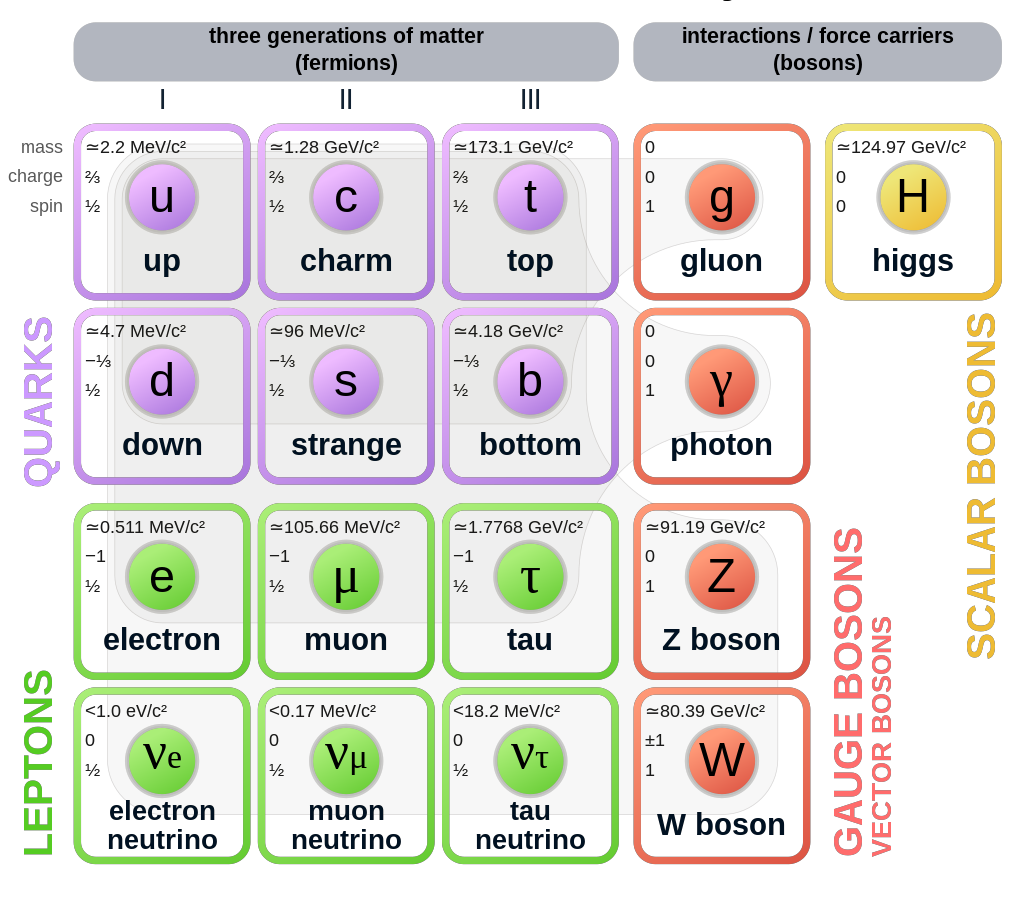
\includegraphics[height=\textwidth]{Standard_Model_of_Elementary_Particles}
        \caption{Standard Model \footnotemark{}}
      \end{figure}
  \end{minipage}\hfill
  \footcitetext{stdmodel}
\end{frame}

\begin{frame}
\frametitle{Standard Model}
\begin{itemize}
\item Fermions: three generations of quarks and leptons
\begin{itemize}
\item Six flavours of quarks: up (u), down (d), charm (c), strange (s), top (t) and bottom (b)
\item Six flavours of leptons: electron ($e$), muon ($\mu$) and tau ($\tau$), and associated neutrinos ($\nu_{e}$, $\nu_{\mu}$ and $\nu_{\tau}$)
\end{itemize}
\item Composite particles: three quark combinations, called baryons ($qqq$/$\bar{q}\bar{q}\bar{q}$) or quark-antiquark pairs, called  mesons ($q\bar{q}$)
\item Mathematically, elementary particles $\rightarrow$ elements of representations of certain symmetry groups
\item Gauge fields coupling to these particles $\rightarrow$ consequence of invariance of corresponding Lagrangian under local phase transformations \footnotemark{}
\item Gauge symmetry that governs the Standard Model is given by: $$SU(3)_{\mathrm{Colour}}\times SU(2)_{\mathrm{Left\ chiral}}\times U(1)_{\mathrm{Y}(\mathrm{Weak \ hypercharge})}$$
\end{itemize}
\footcitetext{thomson_2013}
\end{frame}

\subsection{Electroweak Theory}
\begin{frame}
\frametitle{Electroweak Theory}
\begin{itemize}
\item Initially, EM and the theory of weak interactions formulated separately
\item At higher energies ($\sim$ 246 GeV \footnotemark{}), unified into single force $\rightarrow$ GSW electroweak model - 1960s
\item Impose local gauge invariance on $SU(2)_{L}$ symmetry group $\rightarrow$ three gauge fields: $W^{(1)},\ W^{(2)}$ and $W^{(3)}$
\item Physical $W^{+}$ and $W^{-}$ bosons found to be linear combinations: 
\begin{equation}
W^{\pm}_{\mu}=\dfrac{1}{\sqrt{2}}\left(W^{(1)}_{\mu}\mp \rm{i}W^{(2)}_{\mu}\right)
\end{equation}
\end{itemize}
\footcitetext{pdg-ew}
\end{frame}

\begin{frame}
\frametitle{Electroweak Theory}
\begin{itemize}
\item $W^{(3)}_{\mu}$ field (no physical interpretation ?)
\item Additional symmetry, the $U(1)_{Y}$ group is introduced
\item $B_{\mu}$ field arising from $U(1)_{Y}$ symmetry (no physical meaning ?)
\item Linear combinations of $W^{(3)}_{\mu}$ and $B_{\mu}$ fields $\rightarrow$ photon and the $Z^{0}$ boson:
\begin{equation}
\begin{pmatrix} 
A_{\mu} \\ 
Z_{\mu} 
\end{pmatrix}
= 
\begin{pmatrix}
\cos \theta_{W} & \sin \theta_{W} \\
-\sin \theta_{W} & \cos \theta_{W} 
\end{pmatrix}
\begin{pmatrix}
B_{\mu} \\
W^{(3)}_{\mu}
\end{pmatrix}
\end{equation}
$\theta_{W}$ : weak mixing/Weinberg angle
\end{itemize}
\end{frame}

\subsection{Physics Related to the $Z^{0}$ Resonance}
\subsubsection{Angular Dependence of $\gamma / Z^{0}$ Mediated Processes}
\begin{frame}
\frametitle{Angular Dependence of $\gamma / Z^{0}$ Mediated Processes}
\begin{minipage}{0.5\textwidth}
\begin{itemize}
\item $e^{+}e^{-}\rightarrow e^{+}e^{-}$: t-channel as well as s-channel component
\item $e^{+}e^{-}\rightarrow f\bar{f}$ ($f$ other than $e^{-}$): only s-channel
\end{itemize}
\end{minipage}\hspace{2em}
\begin{minipage}{0.35\textwidth}
      \begin{figure}
      \centering
        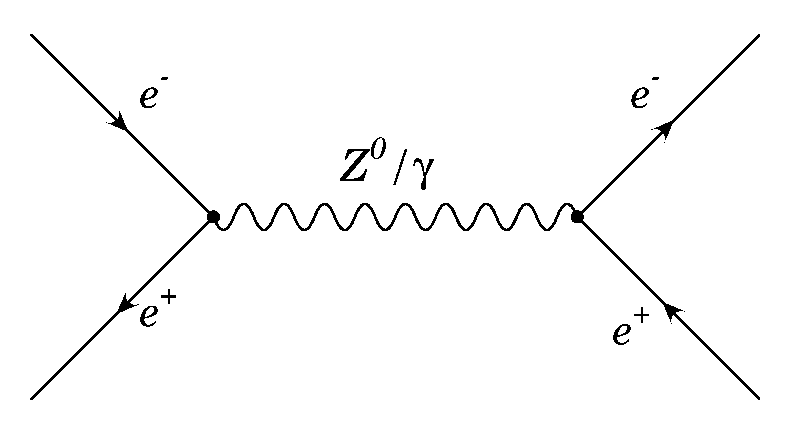
\includegraphics[width=\textwidth]{bhabha-s}
        \caption{$s$-channel Bhaba scattering}
      \end{figure}
      \begin{figure}
      \centering
        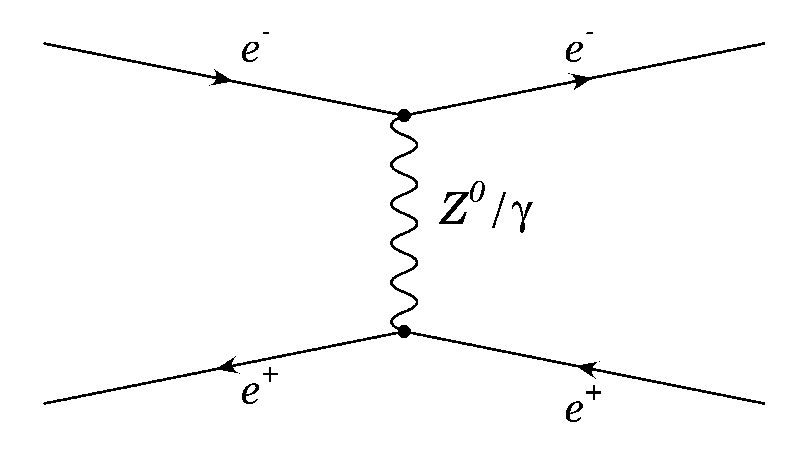
\includegraphics[width=\textwidth]{bhabha-t}
        \caption{$t$-channel Bhaba scattering}
      \end{figure}
  \end{minipage}\hfill
\end{frame}

\begin{frame}
\frametitle{Angular Dependence of $\gamma / Z^{0}$ Mediated Processes}
\begin{minipage}{0.5\textwidth}
\begin{itemize}
\item $s$ channel angular dependence: $\left(\dfrac{d\sigma}{d\Omega}\right)_{s}\propto (1+\cos^{2}\theta)$

Cross section has a major contribution at large angles (or small values of $\cos\theta$)
\item $t$ channel angular dependence: $\left(\dfrac{d\sigma}{d\Omega}\right)_{t}\propto (1-\cos\theta)^{-2}$
Cross section increases asymptotically at small angles (or large values of $\cos\theta$)\footnotemark{}
\item Essential step ! : Remove $t$-channel contribution while finding inherent forward backward asymmetry in $e^{+}e^{-}\rightarrow e^{+}e^{-}$ process
\end{itemize}
\end{minipage}\hspace{1em}
\begin{minipage}{0.45\textwidth}
\begin{figure}
\centering
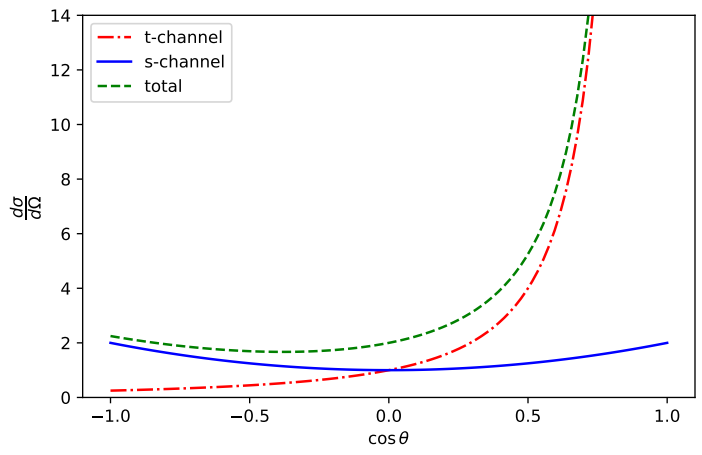
\includegraphics[width=\textwidth]{tangulardist}
\caption{$s$ and $t$-channel angular distribution}
\end{figure}
\end{minipage}\hfill
\footcitetext{UB}
\end{frame}

\subsubsection{Forward-Backward Asymmetry}
\begin{frame}
\frametitle{Forward-Backward Asymmetry}
\begin{itemize}
\item Consider $Z^{0}$ mediated $s$-channel process $e^{+}e^{-}\rightarrow f\bar{f}$
\item Angular dependence:
\vspace{0.5em}
$\left(\dfrac{d\sigma}{d\Omega}\right)_{s\ (Z^{0})}\propto a(1+\cos^{2}\theta) + 2b\cos\theta$
\item No. of fermions in forward dir., ($\theta>\pi /2$) $\neq$ no. of fermions in backward dir., ($\theta<\pi /2$)
\item Asymmetry term $b$: Due to unequal coupling of $Z^{0}$ to right handed and left handed fermions
\vspace{0.5em}
$b=\left[\left(g_{L}^{e}\right)^{2}-\left(g_{R}^{e}\right)^{2}\right]\left[\left(g_{L}^{f}\right)^{2}-\left(g_{R}^{f}\right)^{2}\right]$
\begin{itemize}
\item $g_{L}^{f}$: coupling of $Z^{0}$ to left handed fermions
\item $g_{R}^{f}$: coupling of $Z^{0}$ to right handed fermions
\end{itemize}
\end{itemize}
\end{frame}

\begin{frame}
\frametitle{Forward-Backward Asymmetry}
\begin{itemize}
\item FB asymmetry factor given as the ratio:
\vspace{0.5em}
$\mathcal{A}_{fb}=\dfrac{\sigma_{F}-\sigma_{B}}{\sigma_{F}+\sigma_{B}}=\dfrac{3b}{4a}$
\begin{itemize}
\item $\sigma_{F}, \sigma_{B}$: cross sections in forward and backward directions respectively
\end{itemize}
\item At $Z^{0}$  resonance, $\mathcal{A}_{fb}$ simplifies to \footnotemark{}:
\vspace{0.5em}
$\mathcal{A}_{fb}^{f}\approx 3\left(\dfrac{g_{V}^{f}}{g_{A}^{f}}\right)=1-4\sin^{2}\theta_{W}$
\item From this, ratio of $g_{V}^{f}$ to $g_{A}^{f}$ can be found
\item In turn gives us the Weinberg (weak mixing) angle $\theta_{W}$
\end{itemize}
\footcitetext{thomson_2013}
\end{frame}

\subsubsection{Background Processes: Radiative Corrections}
\begin{frame}
\frametitle{Background Processes: Radiative Corrections}
\begin{minipage}{0.5\textwidth}
\begin{figure}
\centering
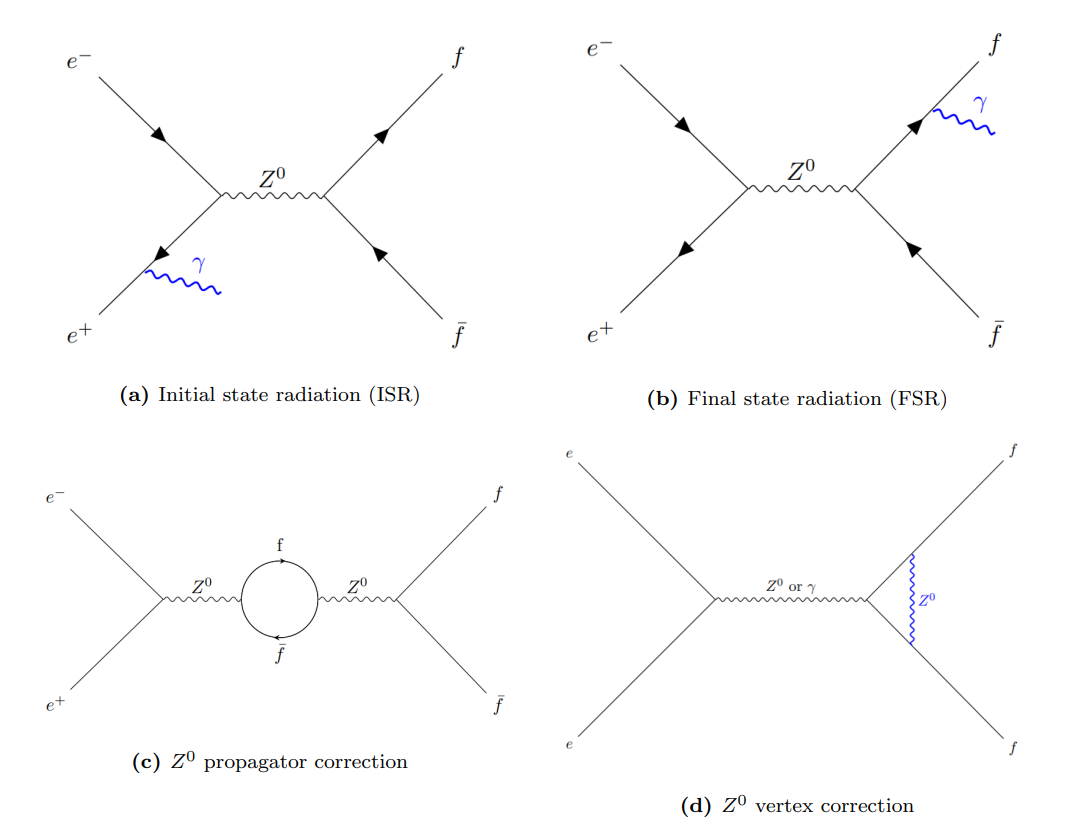
\includegraphics[width=\textwidth]{corrections}
\caption{Some radiative corrections}
\end{figure}
\end{minipage}\hspace{1em}
\begin{minipage}{0.45\textwidth}
To test out predictions of the Standard Model at high precision, need to account for higher order processes \footnotemark{}:
\begin{itemize}
\item \textbf{ISR:} radiation of photons in the initial state $\rightarrow$ decreases $\sqrt{s}$ and affects $Z^{0}$ peak parameters
\item \textbf{FSR:} radiation of photons or gluons in final state $\rightarrow$ partial widths increase
\item \textbf{Electroweak corrections:} Virtual processes like loops in $Z^{0}$ propagator and vertex corrections
\end{itemize}
\end{minipage}\hfill
\footcitetext{Zedometry}
\end{frame}
\subsubsection{Breit Wigner Distribution}
\begin{frame}
\frametitle{Breit Wigner Distribution}
\begin{itemize}
\item Contribution of $Z^{0}$ boson exchange propagator to the matrix element:
\vspace{0.5em}
$\mathcal{M}_{Z^{0}}\propto \dfrac{g_{Z^{0}}^{2}}{q^{2}-m_{Z^{0}}^{2}}=\dfrac{g_{Z^{0}}^{2}}{s-m_{Z^{0}}^{2}}$
\item Around the $Z^{0}$ resonance ($\sqrt{s}\sim  m_{Z^{0}}$), propagator diverges
\item Correction $\rightarrow$ modify propagator for a decaying state
\item For unstable particle having decay rate $\Gamma$, wavefunction modified to:
\vspace{0.5em}
$\psi\propto e^{-imt}\rightarrow e^{-imt}e^{-\Gamma t/2}$
\item Equivalent to introducing an additional imaginary term in the mass:
\vspace{0.5em}
$m\rightarrow m-i\dfrac{\Gamma}{2}$
\item $Z^{0}$ propagator then changes to:
\vspace{0.5em}
$\dfrac{1}{s-m_{Z^{0}}^{2}}\rightarrow \dfrac{1}{s-{\left(m_{Z^{0}}-i\Gamma_{Z^{0}}/2\right)}^{2}}$
\end{itemize}
\end{frame}

\begin{frame}
\frametitle{Breit Wigner Distribution}
\begin{minipage}{0.5\textwidth}
\begin{itemize}
\item Complete form of cross section in process $e^{+}e^{-}\rightarrow Z^{0}\rightarrow f\bar{f}$ is:
\vspace{0.5em}
$\sigma_f (s) = \frac{12\pi}{M_Z^2} \frac{s \Gamma_e \Gamma_f}{(s-M_Z^2)^2 + \left(\frac{s\Gamma_Z}{M_Z}\right)^2} (\hbar^2 c^2)$
\item \textbf{Breit-Wigner distribution:} Probability distribution that characterizes this dependence of cross section on centre of mass energy 
\item Various physical parameters can be extracted by fitting this theoretical distribution to the observed data
\end{itemize}
\end{minipage}\hspace{0.5em}
\begin{minipage}{0.45\textwidth}
\begin{figure}
\centering
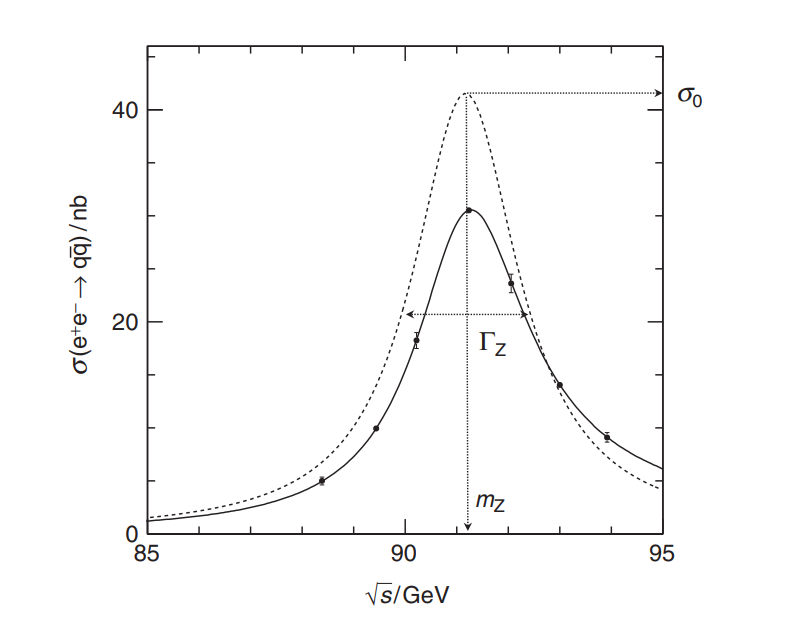
\includegraphics[width=\textwidth]{BWdist}
\caption{Breit Wigner distribution of the cross section for $e^{+}e^{-}\rightarrow q\bar{q}$ process \footnotemark{}}
\end{figure}
\end{minipage}
\footcitetext{thomson_2013}
\end{frame}

\subsubsection{LEP Experiment and OPAL Detector}
\begin{frame}
\frametitle{The LEP Experiment}
\begin{itemize}
\item LEP built at CERN; started operating in 1989
\item One of the major goals: make high precision measurements of $Z^{0}$ boson properties
\item Produced $e^{+}e^{-}$ collisions at $\sqrt{s}$ close to $Z^{0}$ resonance 
\item Recorded about 17 million $e^{+}e^{-}\rightarrow Z^{0}$ events (1989-95) \footnotemark{}
\item Collisions at four different points in the circular collider $\rightarrow$ four detectors:
\begin{itemize}
\item ALEPH (Apparatus for LEP PHysics)
\item DELPHI (DEtector with Lepton, Photon and Hadron Identification)
\item L3 (Third LEP experiment)
\item OPAL (Omni-Purpose Apparatus for LEP)
\end{itemize}
\end{itemize}
\footcitetext{thomson_2013}
\end{frame}

\begin{frame}
\frametitle{OPAL Detector and its Components}
\begin{minipage}{0.5\textwidth}
Starting from origin, as $e^{+}e^{-}$ collision products fly outwards, various detector components are encountered. These are discussed here in brief:
\begin{itemize}
\item \textbf{Vertex detector:} 
\begin{itemize}
\item Surrounds the central beam pipe
\item Key role: locating vertices of short-lived decay products
\item Improves momentum resolution
\end{itemize}
\item \textbf{Jet chamber:}
\begin{itemize}
\item Has good spatial and track resolution
\item Records events associated with jets
\item Also determines $dE/dx$ of charged particles
\end{itemize} 
\end{itemize}
\end{minipage}\hspace{0.5em}
\begin{minipage}{0.45\textwidth}
\begin{figure}
\centering
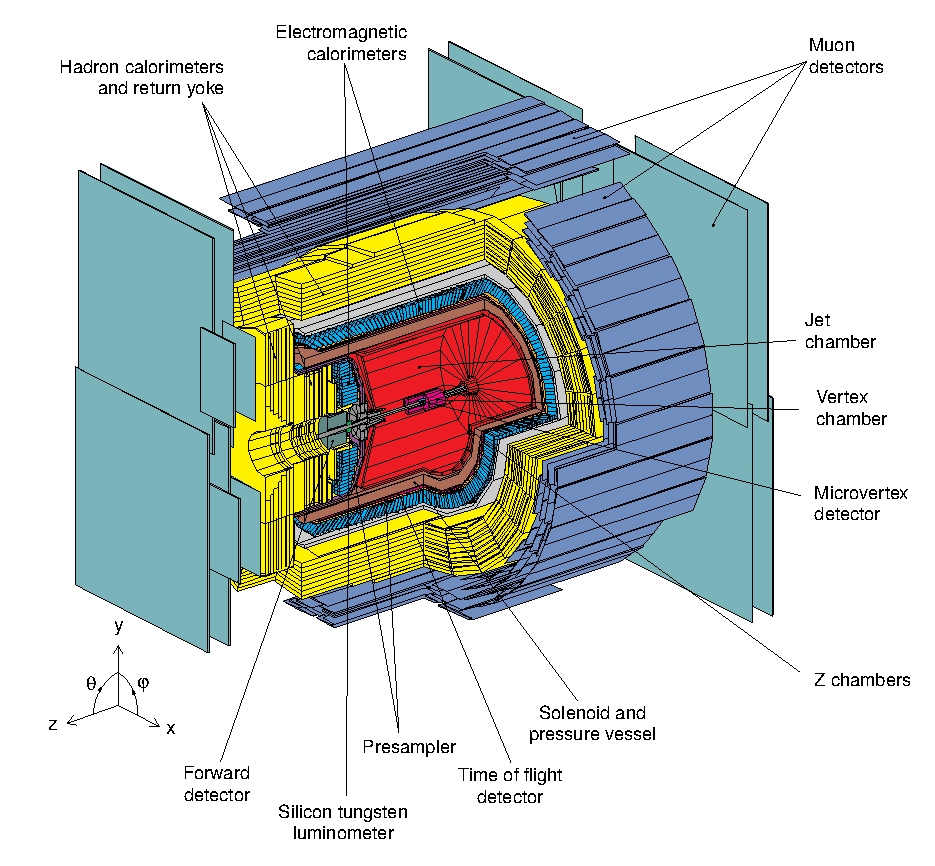
\includegraphics[width=\textwidth]{OPAL1}
\caption{Cross sectional view of the OPAL detector \footnotemark{}}
\end{figure}
\end{minipage}
\footcitetext{OPAL}
\end{frame}

\begin{frame}
\frametitle{OPAL Detector and its Components}
\begin{itemize}
\item \textbf{$\mathbf{z}$ chambers:}
\begin{itemize}
\item Locates $z$ coordinates of decay particles
\item Helpful in improving the resolutions of the polar angle
\end{itemize}
\item \textbf{Solenoid:}
\begin{itemize}
\item Surrounds central detector
\item Generates a uniform magnetic field of 0.435 T along beam dirn.
\item $\vec{B}$ field $\rightarrow$ charged particles have helical path $\rightarrow$ momenta can be measured
\end{itemize}
\item \textbf{ECAL:}
\begin{itemize}
\item $\gamma ,\ e^{-}$ and $e^{+}$ $\xrightarrow[\text{Pair production}]{\text{Bremsstrahlung}}$ deposit all energy in ECAL
\item Hadrons $\rightarrow$ loose some energy (don't stop completely)
\item Lead glass used (high $Z$; entire EM shower contained in small region of space) 
\end{itemize}
\end{itemize}
\end{frame}

\begin{frame}
\frametitle{OPAL Detector and its Components}
\begin{itemize}
\item \textbf{HCAL:}
\begin{itemize}
\item Just like ECAL; detects mesons and baryons
\item Hadronic energy loss : EM shower + strong interaction with nuclei
\item Numerous decay products
\item HCAL occupies more detector volume (significant distance between two consecutive nuclear interactions)
\item Decays more complicated $\rightarrow$ large uncertainty in determining energy loss $\rightarrow$ worse energy resolution compared to ECAL
\end{itemize}
\item \textbf{Muon detector:}
\begin{itemize}
\item Only remaining particles: muons
\item Four layers of muon detectors outside HCAL
\item Provides a coverage of almost the entire solid angle of 4$\pi$ 
\item Has a barrel region and two endcap regions
\end{itemize}
\end{itemize}
\end{frame}

\section{Analysis}
\begin{frame}
\frametitle{Analysis}
\begin{itemize}
  \item Analysis is divided into two parts - Analysis of event displays and Statistical analysis of $Z^0$ decays. 
  \item The main objective of the first part is to understand how different channels affect different observed quantities.
  \item We use this knowledge to come up with cut criteria - a filter to separate out different channels.
  \item The main object of the second part is to use the knowledge from first part and use it to analyse large sets of real world data.
\end{itemize}
\end{frame}

\subsection{Analysis of Event Displays}
\begin{frame}
\frametitle{Analysis of Event Displays}
\begin{itemize}
  \item We analyse event displays of pure events - events of specific channel.
  \item Every event display contains different parameters - number of charged tracks, momentum of all charged tracks, total energy in the EM calorimeter and the total energy in the hadronic calorimeter.
  \item We then plot histograms of different parameteres try to come up with a cut criteria.
  \item Since we already know the behaviour of our detectors to different kinds of particles, we have a rough idea of what to expect.
\end{itemize}
\end{frame}

\begin{frame}
\begin{itemize}
  \item $e^-e^+-$channel: We expect two charged tracks, SumP will have the value of centre of mass energy and all the energy is expected to be deposited in the EM calorimeter and no signal is expected in the hadronic calorimeter.
  \item $\mu^-\mu^+$-channel: Again, two charged tracks, SumP will have the value of centre of mass energy, but no energy depsoited in the calorimeters. Instead, signals in the muon chamber.
  \item $\tau^-\tau^+$-channel: Short life of $\tau$ results in interesting outcomes. We expect to see a large number of charged tracks due to the decay of $\tau$. The dominant decay products are $\mu$ and $\pi$, which can then be detected. This channel can be classified by the number of charge tracks, called prongs.
  \item $q\bar{q}$-channel: Since quarks instantly hadronise, we again have interesting outcomes. The produced hadrons decay further and can be detected. This results in the so-called \textit{jets}, which are much bigger clusters of charged tracks. SumP value is expected to be less than the centre of mass energy, since neutrinos are produced which then carry away some of the energy.
\end{itemize}
\end{frame}

\begin{frame}
\begin{itemize}
  \item We plot histograms of all the quantities to develop cuts.
  \item The bin sizes or chosen so that we are able to see the best possible separation of the different channels.
  \item These cuts are tested on the mixed samples. The mixed samples were classified and checked visually if it matched the channel as determined by the cuts.
\end{itemize}
\begin{table}[h!]
  \centering
  \begin{tabular}{c|cccc}
  \hline
  Channel        & Ctrk(N)          & Ctrk(Sump)        & Ecal(SumE)        & Hcal(SumE)   \\
  \hline
  $e^-e^+$       & (0,6)            &                   & \textgreater{}=80 & \textless{}1 \\
  $\mu^-\mu^+$   & \textless{}6     & \textgreater{}=75 & \textless{}=10    &              \\
  $\tau^-\tau^+$ & \textless{}6     & \textless{}=75    & \textless{}=60    &              \\
  $q\bar{q}$     & \textgreater{}=8 &                   & {[}36,79{]}       &             \\ \hline
  \end{tabular}
  \caption{Cuts determined from event display analysis}
  \label{table:cuts}
\end{table}
\end{frame}

\begin{frame}
\begin{figure}[h!]
  \centering
  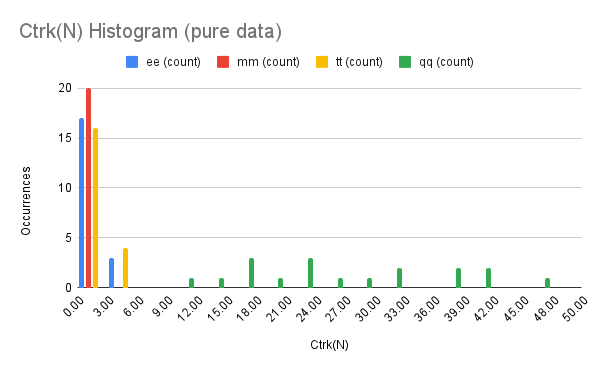
\includegraphics[width = 4cm]{CtrkN-pure.png}
  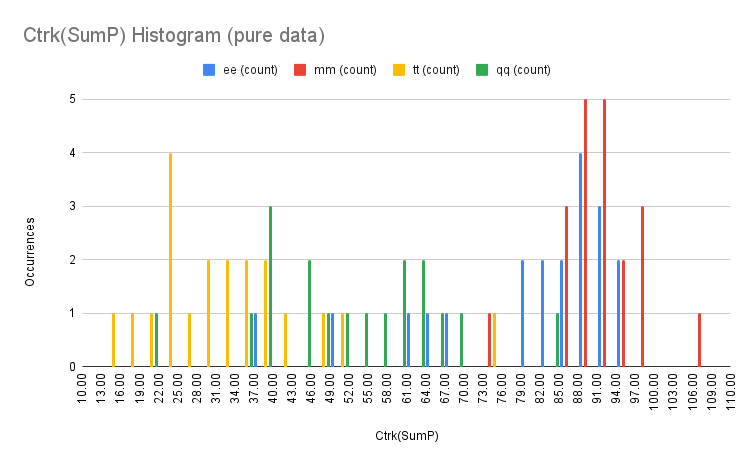
\includegraphics[width = 4cm]{CtrkP-pure.png}
  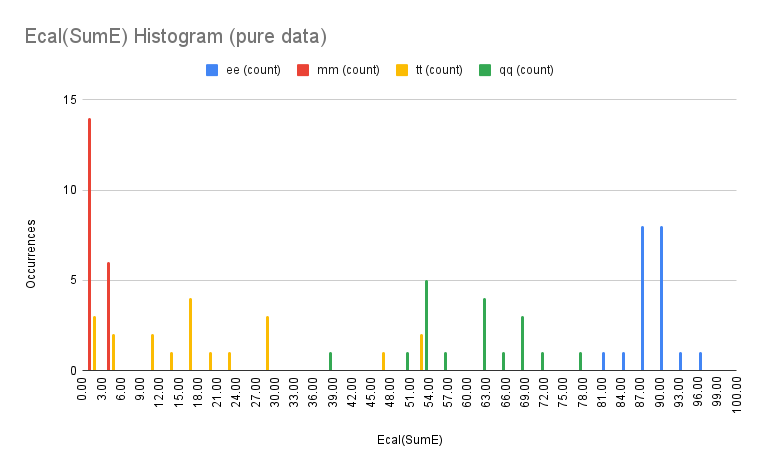
\includegraphics[width = 4cm]{Ecal-pure.png}
  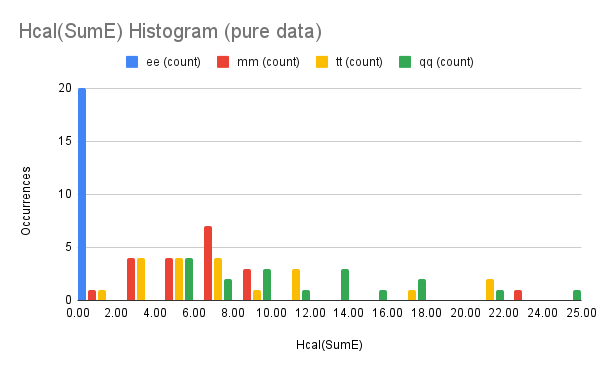
\includegraphics[width = 4cm]{Hcal-pure.png}
  \caption{Histograms of \textit{Ctrk(N)}, \textit{Ctrk(Sump)}, \textit{Ecal(SumE)} and \textit{Hcal(SumE)} for the four channels, generated from \textit{pure} samples.}
  \label{fig:hist}
\end{figure}
\end{frame}

\subsection{Statistical Analysis of $Z^0$ Decays}
\begin{frame}
\frametitle{Statistical Analysis of $Z^0$ Decays}
\begin{itemize}
  \item A simple analysis of event displays is not possible when we have a large number of events. We resort to statistical analysis methods. We use the software, \textit{ROOT} for this purpose.
  \item \textit{ROOT} works with \textit{.root} files, which contain all the information in a tree-like structure, called \textit{ntuple}.
  \item The \textit{ntuple} contains various parameters - run number, event number, number of charged tracks, total scalar sum of track momenta, total energy in the EM calorimeter, total energy in the hadronic calorimeter, LEP beam energy, polar angle beween beam axis and thrust axis, polar angle between incoming positron and outgoing positive particle.
  \item We first use Monte Carlo events to refine our cuts. Then we work with the actual data to calculate different physical quantities.
\end{itemize}
\end{frame}

\begin{frame}
\frametitle{Refining the cuts}
\begin{itemize}
  \item For the $e^-e^+$-channel, we would like to exclude t-channel events. This is because t-channel is possible only in this mode and we omit this for the sake of consistency.
  \item This is achieved by limiting ourselves to smaller angles, since t-channel dominates at large angles. Therefore we take cos$\theta < 0.5$.
  \item But this means that we are excluding some of the s-channel events in this region. The correction factor to account for this, $1.5829$ in our case, is taken from theory.
  \item For the $\mu^-\mu^+$-channel, we observed a lot of events with scalar momenta exactly equal to zero. These are not physical and we ignore them by modifying our cuts.
  \item For the above two channels, we also modified our cuts to ignore angles very close to the beam axis, since the resolution of our detector is far from perfect in that region.
  \item The other two channels did not require any additional cut, but we did need cos$\theta$ to take only the values between $-1$ and $1$ to exclude unphysical events.
\end{itemize}
\end{frame}

\begin{frame}
\frametitle{Efficiency matrix}
\begin{itemize}
  \item We now begin our ultimate analysis. We used \textit{data6.root} in our analysis.
  \item Our cuts are not perfect. Ideally, the cuts should completely separate out every channel perfectly, but this is not the case.
  \item To account for this, we use efficiency matrix. Efficiency matrix, as the name suggests, is a measure of how efficient our cuts are.
  \item It is given by,
  \begin{equation}
    \epsilon_{ij} = \frac{N^{i, cut}_j}{N^{j, all}_j}.
  \end{equation}
  \item This translates to i-th cut applied to j-th channel divided by the total number of j-th channel events. This then gives the actual counts as,
  \begin{equation}
    N_{obs} = \epsilon N_{actual} \implies N_{actual} = \epsilon^{-1} N_{obs}.
  \end{equation}
  \item To summarise, we start with the observed counts with our cuts, understand that this is not the true counts and we use the efficiency matrix to calculate the true counts.
  \item The efficiency matrix can be found in the report. The true counts are used for all our calculations.
\end{itemize}
\end{frame}

\begin{frame}
\frametitle{Cross Sections}
\begin{itemize}
  \item With the actual counts, we can calculate the cross section values.
  \item This is given by,
  \begin{equation}
    \sigma = \frac{N_{actual}}{\int \mathcal{L} dt} + \text{cf(radiation)}.
  \end{equation}
  \item The term $\int \mathcal{L} dt$ is the integrated luminosity and cf(radiation) is the radiative correction factor, the values for which are taken from \footnotemark{}.
  \item We get the following cross section values,
  \begin{table}[!h]
    \centering
    \begin{tabular}{c|cccc}
    \hline
    $\sqrt{s}$ {[}GeV{]} & $\sigma_{ee}$ {[}nb{]} & $\sigma_{mm}$ {[}nb{]} & $\sigma_{tt}$ {[}nb{]} & $\sigma_{qq}$ {[}nb{]} \\
    \hline
    88.47                & 0.39 $\pm$ 0.03        & 0.30 $\pm$ 0.02        & 0.47 $\pm$ 0.03        & 7.19 $\pm$ 0.10        \\
    89.46                & 0.82 $\pm$ 0.04        & 0.65 $\pm$ 0.03        & 0.72 $\pm$ 0.03        & 14.20 $\pm$ 0.14       \\
    90.22                & 1.26 $\pm$ 0.04        & 1.16 $\pm$ 0.03        & 1.12 $\pm$ 0.03        & 25.70 $\pm$ 0.21       \\
    91.22                & 1.69 $\pm$ 0.02        & 1.82 $\pm$ 0.02        & 1.75 $\pm$ 0.02        & 40.75 $\pm$ 0.22       \\
    91.97                & 1.12 $\pm$ 0.05        & 1.32 $\pm$ 0.04        & 1.21 $\pm$ 0.04        & 28.96 $\pm$ 0.27       \\
    92.96                & 0.45 $\pm$ 0.04        & 0.55 $\pm$ 0.03        & 0.66 $\pm$ 0.04        & 13.67 $\pm$ 0.20       \\
    93.71                & 0.28 $\pm$ 0.03        & 0.34 $\pm$ 0.02        & 0.40 $\pm$ 0.03        & 8.20 $\pm$ 0.13       \\
    \hline
    \end{tabular}
    \caption{Calculated cross section values for different $\sqrt{s}$ values.}
    \label{table:cross-section}
  \end{table}
\end{itemize}
\footcitetext{UB}
\end{frame}

\begin{frame}
\frametitle{Forward Backward Asymmetry and Weak Mixing Angle}
\begin{itemize}
  \item As discussed in the theory section, $Z^0$ couples differently to left- and right-handed fermions, which leads to an asymmetry in the angular distribution of the final state particles.
  \item This asymmetry depends on the weak mixing angle. Therefore, by calculating this simple asymmetry we can calculate the weak mixing angle.
  \item We perform this calculation for the $\mu^-\mu^+$ channel, since we do not have the issue of t-channel and we also get two clear tracks.
  \item The forward backward asymmetry is given by,
  \begin{equation}
    A_{fb} = \frac{N_+ - N_-}{N_+ + N_-} + \text{cf($A_{fb}$)}.
  \end{equation}
  \item cf(A$_{fb}$) are the correction factors corresponding to forward bacward asymmetry, the values for which are taken from \footnotemark{}.
\end{itemize}
\footcitetext{UB}
\end{frame}

\begin{frame}
\begin{itemize}
  \item A$_{fb}$ is then used to calculate the weak mixing angle. We get $sin^2\theta_W = 0.2369 \pm 0.0085$ for the data event at resonance energy and $sin^2\theta_W = 0.2352 \pm 0.0098$ for the MC event.
  \item The literature value is $sin^2\theta_W = 0.2352 \pm 0.0098$ \footnotemark{}, which is withing one standard deviation of both our results.
\end{itemize}
\footcitetext{pdg2}
\end{frame}

\begin{frame}
\frametitle{Lepton Universality}
\begin{itemize}
  \item Since the masses of leptons are much smaller compared to that of the $Z^0$, the cross sections of all the three leptonic decay modes must be the same at resonance.
  \item We see that, at resonance, the cross sections are given by,
  \begin{equation}
    \begin{split}
        \sigma_e = 1.69 \pm 0.02 \text{nb} \\
        \sigma_{\mu} = 1.82 \pm 0.02 \text{nb} \\
        \sigma_{\tau} = 1.75 \pm 0.02 \text{nb}
    \end{split}
  \end{equation}
  \item The theoretical value is $\sigma_f = 1.99$nb. The values we have calculated are several standard deviations away, unfortunately. But they are roughly the same and match up to the order.
  \item We postulate that this is because we don't have the best possible cut criteria. We are undercounting the event numbers to some extent and since this is a very sensity quatity, it gets affected significantly.
  \item We suggest that we increase the number of events significantly, to improve statistical accuracy.
\end{itemize}
\end{frame}

\begin{frame}
\begin{itemize}
  \item The ratios of hadronic to the leptonic modes follow a similar discrepancy,
  \begin{equation}
    \begin{split}
        \frac{\sigma_{had}}{\sigma_e} = 24.18 \pm 0.30 \\
        \frac{\sigma_{had}}{\sigma_{\mu}} = 22.43 \pm 0.24 \\
        \frac{\sigma_{had}}{\sigma_{\tau}} = 23.28 \pm 0.26
    \end{split}
  \end{equation}
  \item The literature value is $20.804 \pm 0.050$, $20.785 \pm 0.033$ and $20.764 \pm 0.045$ respectively \footnotemark{}.
\end{itemize}
\footcitetext{pdg2}
\end{frame}

\begin{frame}
\frametitle{Breit-Wigner Fit of Cross Sections}
\begin{itemize}
  \item We now extract the all important quantities from our data. We do this by fitting our cross sections to a Breit-Wigner curve.
  \item The curve is given by,
  \begin{equation}
    \sigma_f (s) = \frac{12\pi}{M_Z^2} \frac{s \Gamma_e \Gamma_f}{(s-M_Z^2)^2 + \left(\frac{s\Gamma_Z}{M_Z}\right)^2} (\hbar^2 c^2).
  \end{equation}
  \item This has three parameters, $M_Z$, $\Gamma_Z$ and $\Gamma_e\Gamma_f$. The factor $\hbar^2 c^2$ is used to convert the cross section values to SI units from natural units.
  \item We see that we can extract the physical quantities we are interested in, from the fit parameters.
  \item We used \textit{scipy.optimize} module for \textit{Python3} to fit our curve against the data. We calculated the follwing parameters for our fits,
  \begin{table}[h!]
    \centering
    \begin{tabular}{c|ccc}
    \hline
    Channel        & $M_Z$ {[}GeV{]}    & $\Gamma_Z$ {[}GeV{]} & $\Gamma_e\Gamma_f$ {[}GeV$^2${]}                    \\ \hline
    $e^-e^+$       & 90.973 $\pm$ 0.047 & 2.591 $\pm$ 0.158    & 6.615$\times$10$^{-3}$ $\pm$ 6.29$\times$10$^{-4}$ \\
    $\mu^-\mu^+$   & 91.117 $\pm$ 0.021 & 2.462 $\pm$ 0.060    & 6.306$\times$10$^{-3}$ $\pm$ 2.46$\times$10$^{-4}$ \\
    $\tau^-\tau^+$ & 91.159 $\pm$ 0.058 & 2.825 $\pm$ 0.179    & 7.690$\times$10$^{-3}$ $\pm$ 7.85$\times$10$^{-4}$ \\
    $q\bar{q}$     & 91.187 $\pm$ 0.004 & 2.515 $\pm$ 0.010    & 0.1460 $\pm$ 0.0009                                \\ \hline
    \end{tabular}
    \caption{Fit parameters and reduced $\chi^2$ values for the data}
    \label{table:bwfit}
  \end{table}
\end{itemize}
\end{frame}

\begin{frame}
\begin{itemize}
  \item The reduced $chi^2$ value for our fits are $3.47$, $1.10$, $8.34$ and $0.58$ respectively.
  \item Note that a reduced $\chi^2$ value of less than $1$ implies we are over-fitting our data or the error variances are overestimated, whereas values greater than $1$ implies the opposite.
  \item If the reduced $\chi^2$ values is much greater than $1$, it means that we have a bad fit. But we also note that none of our fits have a corresponding $p-value$ less than $0.05$.
\end{itemize}
\end{frame}

\begin{frame}
  \begin{figure}[h!]
    \begin{center}
        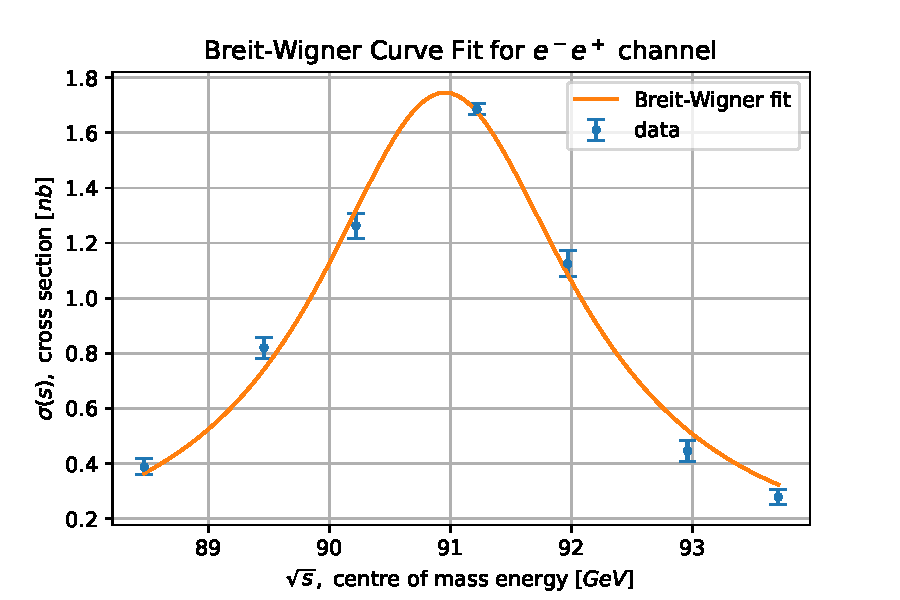
\includegraphics[width = 4 cm]{e213-ee-fit.pdf}
        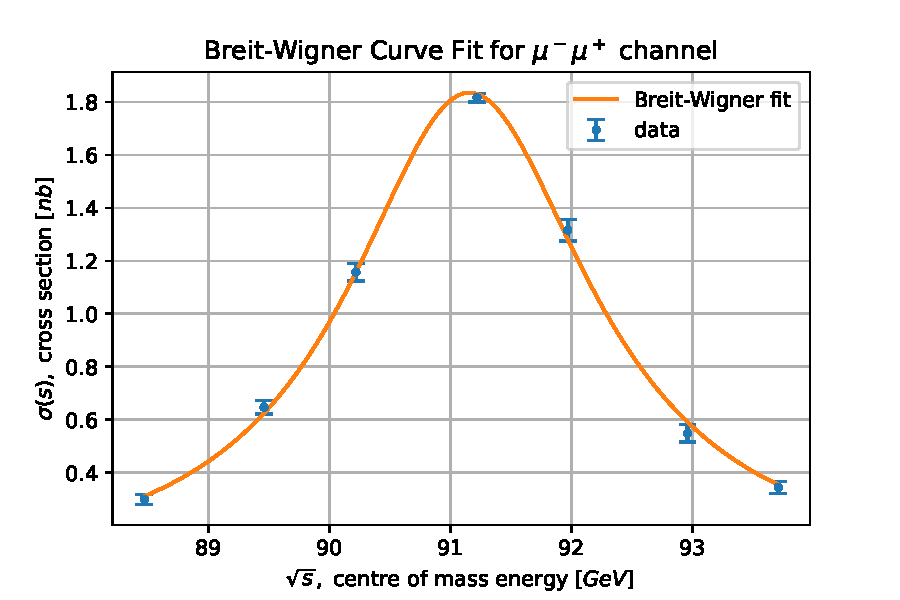
\includegraphics[width = 4 cm]{e213-mm-fit.pdf}
        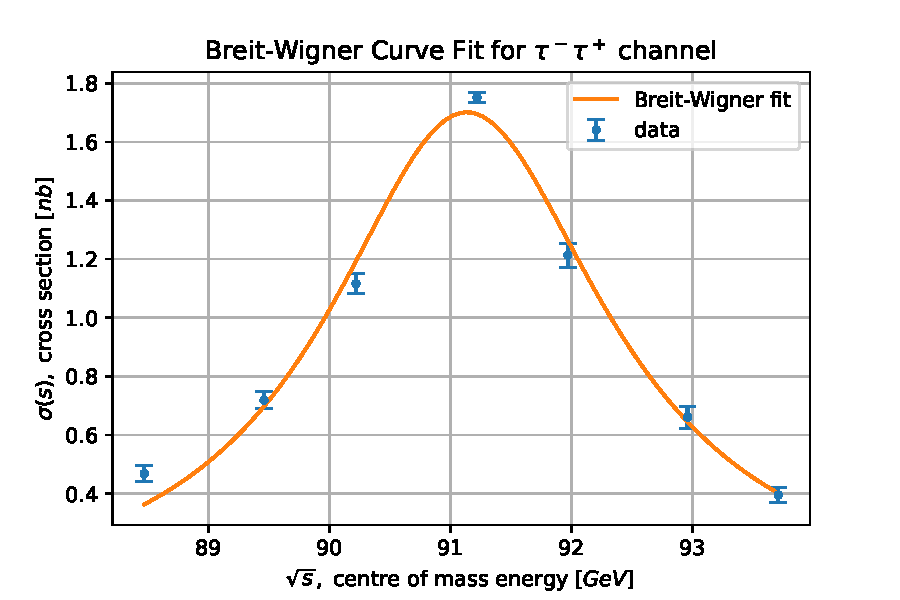
\includegraphics[width = 4 cm]{e213-tt-fit.pdf}
        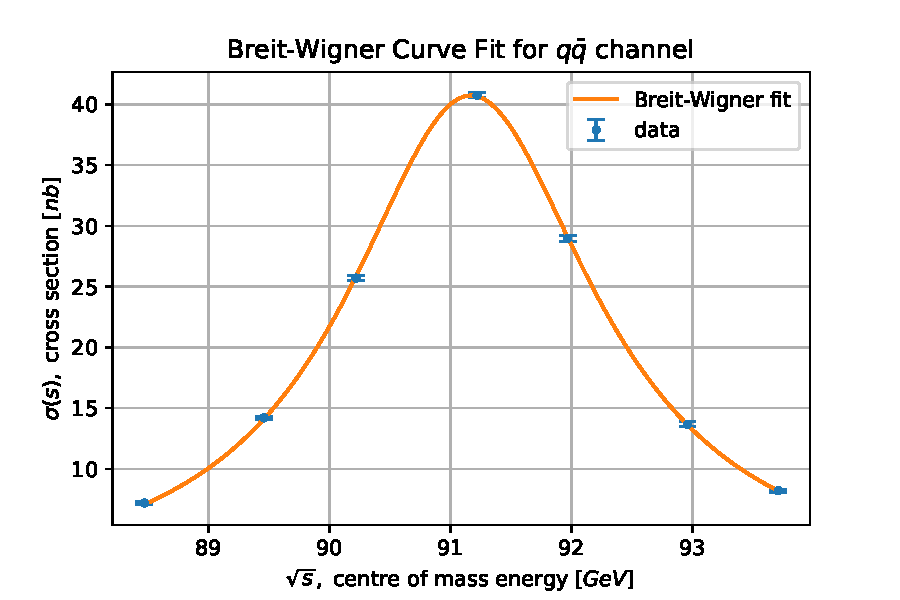
\includegraphics[width = 4 cm]{e213-qq-fit.pdf}
    \end{center}
    \caption{Breit-Wigner fit for the four different decay channels}
    \label{fig:bwfit}
    \end{figure}
\end{frame}

\begin{frame}
\begin{itemize}
  \item From the fit parameters, we calculate,
  \begin{equation}
    \begin{split}
        M_Z = 91.123 \pm 0.020 \\
        \Gamma_Z = 2.598 \pm 0.062.
    \end{split}
  \end{equation}
  \item The literature values are $M_Z = 91.1876 \pm 0.0021$ and $\Gamma_Z = 2.4952 \pm 0.0023$ \footnotemark{}.
  \item The literature value for $M_Z$ lies within $4\sigma$ of our calculated value, whereas the literature value for $\Gamma_Z$ lies within $2\sigma$ of our calculated value.
  \item We also note that the literature value for $M_Z$ lies within one standard deviation of the value obtained from the $q\bar{q}$ fit, which had the most counts.
  \item This hints us that we could improve our accuracy of the results by significantly increasing the number of events analysed.
\end{itemize}
\footcitetext{pdg2}
\end{frame}

\begin{frame}
\frametitle{Partial Width of Different Channels and Number of Light Neutrino Generations}
\begin{itemize}
  \item We can calculate the partial width from the third fit parameter. We calculate,
  \begin{table}[h!]
    \centering
    \begin{tabular}{c|cc}
    \hline
    Channel        & $\Gamma_f$ {[}MeV{]} & $\Gamma_f$ (lit.) {[}MeV{]} \\ \hline
    $e^-e^+$       & 81.33 $\pm$ 5.47     & 83.91 $\pm$ 0.12              \\
    $\mu^-\mu^+$   & 77.53 $\pm$ 6.03     & 83.99 $\pm$ 0.18              \\
    $\tau^-\tau^+$ & 94.56 $\pm$ 11.55    & 84.08 $\pm$ 0.22              \\
    $q\bar{q}$     & 1795.52 $\pm$ 121.31 & 1744.4 $\pm$ 2.0              \\ \hline
    \end{tabular}
    \caption{Partial decay width of different channels and literature values}
    \label{table:decaywidth}
  \end{table}
  \item The literature values \footnotemark{} lie within one standard deviation of the calculated partial width, which is impressive.
  \item But we also note that the precision of our results is not as good as the literature value precision.
  \item How precise the value of $\Gamma_f$ is, ultimately depends on the precision of the cross section values, which can be improved only by observing more events.
\end{itemize}
\footcitetext{pdg2}
\end{frame}

\begin{frame}
\begin{itemize}
  \item We now determine the number of generations of light neutrinos using,
  \begin{equation}
    n_{\nu} = \frac{\Gamma_Z - \Gamma_e - \Gamma_{\mu} - \Gamma_{\tau} - \Gamma_q}{\Gamma_{\nu}}.
  \end{equation}
  \item This gives the number of neutrino generations as $3.28 \pm 0.45$. We have used the value for $\Gamma_{\nu}$ from \footnotemark{}.
  \item This tells us that number of neutrino generations are $3$. And within one standard deviation, our result absolutely excludes the possibility of fourth neutrino generation.
\end{itemize}
\footcitetext{UB}
\end{frame}

\section{Discussion \& Conclusion}
\begin{frame}
\frametitle{Discussion \& Conclusion}
\begin{itemize}
  \item Our objective to understand how analysis is carried out with data from a particle collider was achieved in this experiment.
  \item We do not have information about uncertainties associated with different components of the detector. This systematic error is not accounted for, in our calculations.
  \item Certain quantities, like radiative corrections, did not contain any uncertainties \footnotemark{}. This would contribute to the overall error.
  \item We calculated quantities like the cross sections, weak mixing angle, the mass and decay width of $Z^0$ boson and its partial decay width, all from the particle counts at different centre of mass energies.
  \item We also compared the accuracy of these quantities with the literature values.
  \item We calculated the maximum possible light neutrino generations and eliminated the possibility of a fourth generation.
  \item All this analysis ultimately relied on the measurement of $N$, which implies that we could improve both the accuracy and precision of the results by significantly increasing $N$.
\end{itemize}
\footcitetext{UB} 
\end{frame}

\section*{References}
\begin{frame}
\frametitle{References}
\printbibliography
\end{frame}
\end{document}